\documentclass{standalone}
%<--------------------------------------------------------------------------->%
%%% Color %%%
\usepackage[dvipsnames]{xcolor} % \textcolor{red}{}
\definecolor{rot}{RGB}{229,0,0}
\definecolor{bla}{RGB}{0,98,144}
\definecolor{gel}{RGB}{255,195,0}
%<--------------------------------------------------------------------------->%

%<--------------------------------------------------------------------------->%
%%% TikZ %%%
\usepackage{tikz}
\usetikzlibrary{calc}
% \usetikzlibrary{fit}
\usetikzlibrary{angles,quotes}
% \usetikzlibrary{intersections,topaths}
% \usetikzlibrary{decorations.markings}
%<--------------------------------------------------------------------------->%
%%% TikZ: Mark Angles %%%
\newcommand{\MarkRightAngle}[5][]{%
\draw[#1] let \p1=($(#3)-(#4)$),\n1={1/veclen(\x1,\y1)},\p2=($(#4)-(#5)$),\n2={1/veclen(\x2,\y2)}in%
($(#4)!#2!(#5)$) -- ++(\x1*\n1*#2,\y1*\n1*#2) -- ++(\x2*\n2*#2,\y2*\n2*#2);}
\newcommand{\MarkAngle}[5]["$\theta$",->,draw=blue!80,fill=blue!20]{\pic[#1,angle radius=#2] {angle = #3--#4--#5};}
%<--------------------------------------------------------------------------->%

\begin{document}

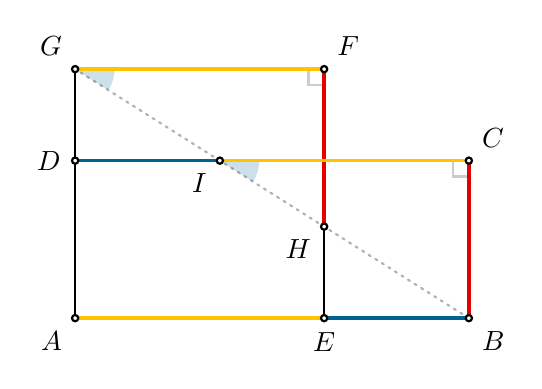
\begin{tikzpicture}[thick,line cap=round]
	\tikzstyle{jiao}=[solid,circle,draw,fill=white,inner sep=.8pt];
	\tikzstyle{rightangle}=[opacity=0.2];
\newcommand{\rightanglesize}{0.2cm}
\tikzstyle{normalangle}=[fill=bla,opacity=0.2];
\newcommand{\anglesize}{0.5cm}
\tikzstyle{help}=[dotted,opacity=0.2];
%<--------------------------------------------------------------------------->%

	\newcommand{\width}{5cm}
	\newcommand{\height}{2cm}
	\newcommand{\square}{{sqrt(\width*\height)}}
	\coordinate (A) at (0,0);
	\coordinate (B) at (\width,0);
	\coordinate (C) at (\width,\height);
	\coordinate (D) at (0,\height);
	\coordinate (E) at (\square,0);
	\coordinate (F) at (\square,\square);
	\coordinate (G) at (0,\square);
	\coordinate (H) at ($(F)-(0,\height)$);
	\coordinate (I) at ($(C)-(\square,0)$);
	\draw (A) rectangle (C);
	\draw (A) rectangle (F);
	\draw[opacity=0.3,dotted] (B) -- (G);
	%% Final
	\MarkAngle[normalangle]{\anglesize}BIC;
	\MarkAngle[normalangle]{\anglesize}HGF;
	\MarkRightAngle[rightangle]{\rightanglesize}ICB;
	\MarkRightAngle[rightangle]{\rightanglesize}GFH;
	\draw[very thick,rot] (F) -- (H);
	\draw[very thick,rot] (B) -- (C);
	\draw[very thick,gel] (F) -- (G);
	\draw[very thick,gel] (I) -- (C);
	\draw[very thick,gel] (A) -- (E);
	\draw[very thick,bla] (E) -- (B);
	\draw[very thick,bla] (D) -- (I);
	\node[jiao,label=below left  :{$A$}] at (A) {};
	\node[jiao,label=below right :{$B$}] at (B) {};
	\node[jiao,label=above right :{$C$}] at (C) {};
	\node[jiao,label=left        :{$D$}] at (D) {};
	\node[jiao,label=below       :{$E$}] at (E) {};
	\node[jiao,label=above right :{$F$}] at (F) {};
	\node[jiao,label=above left  :{$G$}] at (G) {};
	\node[jiao,label=below left  :{$H$}] at (H) {};
	\node[jiao,label=below left  :{$I$}] at (I) {};
\end{tikzpicture}

\end{document}
